\chapter{Background}
\section{Whole Slide Image Formats}
As the size of an acquired raw, uncompressed WSI is massive\footnote{ A typical 1,600 megapixel slide requires about 4.6 GB of memory on average\cite{Farahanil15}. The size of a H\&E (hematoxylin and eosin) stained slide ranges typically from 4 to 20 GB\cite{Singh11}.}, file formatting is required to mitigate the enormous amounts of information. Since there is no standardized format for WSIs, vendors came up with their own, proprietary solutions, which vary greatly\cite{Cornish13}. Efforts of standardization are being made through the \emph{Digital Imaging and Communications in Medicine} (DICOM) Standard\cite{DICOM10}\nmc{DICOM}{Digital Imaging and Communications in Medicine}.

Usually, WSI files are stored as a multitude of single images, spanning multiple folders and different resolutions. Those files are used to construct a so called \emph{image pyramid}\cite{Farahanil15} (see fig. 2.1 and the following DICOM Supplement 145 subsection).


\subsubsection{DICOM Supplement 145}
\cite{Singh11} describes DICOM as follows:
\begin{quotation}
	"Digital Imaging and Communications in Medicine (DICOM), synonymous with ISO (International Organization for Standardization) standard 12052, is the global standard for medical imaging and is used in all electronic medical record systems that include imaging as part of the patient record."
\end{quotation}

Before \emph{Supplement 145: Whole Slide Microscopic Image IOD and SOP Classes}, the DICOM Standard did not address standardization of WSI. Among others, the College of American Pathologist’s Diagnostic Intelligence and Health Information Technology Committee is responsible for the creation and further advancement of this supplement\cite{Singh11}.

It addresses every step involved in creating WSIs: image creation, acquisition, processing, analyzing, distribution, visualization and data management\cite{DICOM10}. It impacted the way how data is stored greatly\cite{Singh11}, due to the introduction of a pyramid image model\cite{DICOM10} (see fig. 2.1).

\begin{figure}[H]
	\begin{center}
		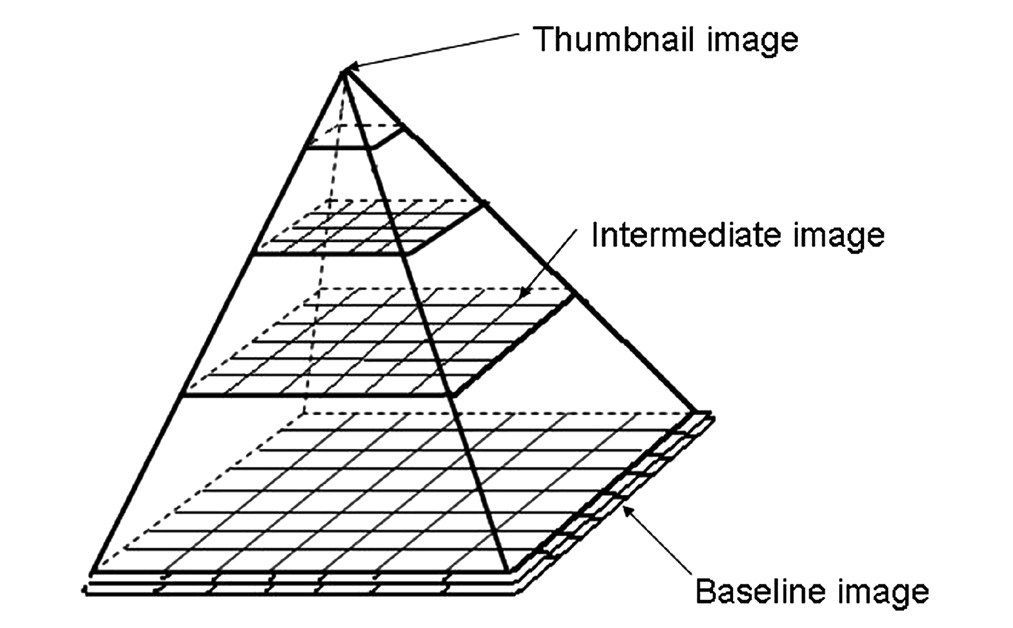
\includegraphics[scale=0.2]{img/imgPyramid.png}
		\caption{DICOMs image pyramid (source:\cite{Singh11})}
		\label{fig:fig2.1}
	\end{center}
\end{figure}

The image pyramid model facilitates rapid zooming and reduces the computational burden of randomly accessing and traversing a WSI\cite{Singh11},\cite{Park12}. This is made possible by storing an image in several precomputed resolutions, with the highest resolution sitting at the bottom (called the \emph{baseline image}) and a thumbnail or low power image at the top (compare fig. 2.1)\cite{DICOM10}. This creates a pyramid like stack of images, hence the name "pyramid model". The different resolutions are referred to as \emph{layers}\cite{DICOM10} or \emph{levels}\cite{Singh11} respectively.

Each level is tessellated into square or rectangular fragments, called tiles, and stored in a two dimensional array\cite{Farahanil15}. 

Because of this internal organization, the tiles of each level can be retrieved and put together separately, to either form a subregion of the image or show it entirely. This makes it easy to randomly access any subregion of the image without loading large amounts of data\cite{Singh11}.


\subsection{Proprietary Formats}
Vendors of whole slide scanners implement their own file formats, libraries and viewers (see tab. 2.1 for a list of vendors and their formats). Because of this, they can focus on the key features and abilities of their product. This generally leads to a higher usability, ease-of-use and enables highly tailored customer support. Furthermore, in comparison to open source projects, the longevity of proprietary software is often higher\cite{Optimus15}.

\begin{table}[H]
	\begin{center}
		\begin{tabular}{| l | l |}
			\hline
			\textbf{vendor} & \textbf{formats}\\ \hline
			Aperio & SVS, TIF\\ \hline
			Hamamatsu & VMS, VMU, NDPI\\ \hline
			Leica & SCN\\ \hline
			3DHistech/Mirax & MRXS\\ \hline
			Philips & TIFF\\ \hline
			Sakura & SVSLIDE\\ \hline
			Trestle & TIF\\ \hline
			Ventana & BIF, TIF\\ \hline
		\end{tabular}
		\caption{File formats by vendor}
	\end{center}
\end{table}

Since the proprietary formats have little to no documentation, most of the information presented here was reverse engineered in \cite{Goode13} and \cite{web:openslide}. All proprietary formats listed here implement a modified version of the pyramid model introduced in \cite{DICOM10}.


\subsubsection{Aperio}
The SVS format by Aperio is a TIFF-based format, which comes in a single file\cite{Goode13}. It has a specific internal organization in which the first image is the baseline image, which is always tiled (usually with 240x240 pixels). This is followed by a thumbnail, typically with dimensions of about 1024x768 pixels. The thumbnail is followed by at least one intermediate pyramid image (compare fig. 2.1), with the same compression and tile organization as the baseline image\cite{web:openslide}. Optionally, there may be a slide label and macro camera image at the end of each file\cite{web:openslide}.


\subsubsection{Hamamatsu}
Hamamatsu WSIs come in 3 variants:
\begin{enumerate}[(1)]
	\item VMS
	\item VMU
	\item NDPI
\end{enumerate}

(1) and (2) consist of an index file ((1) - [file name].vms, (2) - [file name].vmu) and 2 or more image files. In the case of (2), there is also an additional optimization file. (3) consists of a single TIFF-like file with custom TIFF tags. While (1) and (3) contain jpeg images, (2) contains a custom, uncompressed image format called \emph{NGR}\footnote{For more information on NGR, consult \url{http://openslide.org/formats/hamamatsu/}}\cite{web:openslide}.

The random access support for decoding parts of jpeg files is poor. To get around this, so called \emph{restart markers}\footnote{Restart markers were originally designed for error recovery. The markers allow the decoder to resynchronize at set intervals throughout the image\cite{Goode13}.} are used to create virtual slides\cite{Goode13}. The markers are placed at regular intervals. The offset of every marker is specified in different manner. In the case of (1), it can be found in the index file. In the case of (2), the optimization file holds the information and in the case of (3), a TIFF tag contains the offset\cite{web:openslide}.


\subsubsection{Leica}
SCN is a single file format based on BigTIFF, additionally .scn provides a pyramidal thumbnail image.\cite{Goode13}.

The first TIFF directory has a tag called "ImageDescription" which contains an XML document that defines the internal structure of the WSI\cite{web:openslide}.

Leica WSIs are structured as a collection of images, each of which has multiple pyramid levels. While the collection only has a size, images have a size and position, all measured in nanometers. Each dimension has a size in pixels, an optional focal plane number, and a TIFF directory containing the image data. Fluorescence images have different dimensions (and thus different TIFF directories) for each channel\cite{web:openslide}.

Brightfield slides have at least two images: a low-resolution macro image and one or more main images corresponding to regions of the macro image. Fluorescence slides can have two macro images: one brightfield and one fluorescence\cite{web:openslide}.


\subsubsection{3DHistech/Mirax}
MRXS is a multi-file format with very complicated metadata in a mixture of text and binary formats. Images are stored as either JPEG, PNG or BMP\cite{Goode13}. The poor handling of random access is also applicable to PNG. Because of this, multiple images are needed to encode a single slide image. To avoid having many individual files, images are packed into a small number of data files. An index file provides offsets into the data files for each required piece of data.\cite{web:openslide}. 

A 3DHistech/Mirax scanner take images with an overlap. Each picture taken is then tessellated without an overlap. Therefore, they only occur between taken pictures\cite{web:openslide}.

The generation of the image pyramid differs from the process described in 2.1. To create the $n^{th}$ level, each image of the $n^{th}-1$ level is divided by 2 in each dimension and then concatenated into a new image. Where the $n^{th}-1$ level had 4 images in 2x2 neighborhood, the $n^{th}$ level will only have 1 image. This process has no regards for overlaps. Thus, overlaps may occur in the higher levels of the image pyramid\cite{web:openslide}.


\subsubsection{Philips}
Philips' TIFF is an export from the native iSyntax format. An XML document with the hierarchical structure of the WSI can be found over the \emph{ImageDescription} tag of the first TIFF directory. It contains key-value pairs based on DICOM tags\cite{web:openslide}.

Slides with multiple regions of interest are structured as a single image pyramid enclosing all regions. Slides may omit pixel data for TIFF tiles not in an ROI. When such tiles are downsampled into a tile that does contain pixel data, their contents are rendered as white pixels\cite{web:openslide}.

Label and macro images are stored either as JPEG or as stripped TIFF directories.


\subsubsection{Sakura}
WSIs in the SVSLIDE format are SQLite 3 database files. Their tables contain the metadata, associated images and tiles in the JPEG format. The tiles are addressed as (focal plane, downsample, level-0 X coordinate, level-0 Y coordinate, color channel). Additionally, each color channel has a separate grayscale image\cite{web:openslide}.


\subsubsection{Trestle}
Trestles TIF is a single-file TIFF. The WSI has the standard pyramdic scheme and tessellation. It contains non-standard metadata and overlaps, which are specified in additional files. The first image in the TIFF file is the baseline image. Subsequent images are assumed to be consecutive levels of the image pyramid with decreasing resolution\cite{web:openslide}.


\subsubsection{Ventana}
Ventanas WSIs are single-file BigTIFF images, organized in the typical pyramidical scheme. The images are tiled and have non-standard metadata, as well as overlaps. They come with a macro and a thumbnail image\cite{web:openslide}.

	
\subsection{Open Formats}
As mentioned in 2.1.1, proprietary formats typically come without much or any documentation. Furthermore, a vendors viewer is usually the only way of viewing WSIs of a particular format. This creates a vendor lock-in, where users can't take advantage of new improvements offered by other vendors. Furthermore, most viewers only provide support for Windows platforms. While, in a clinical setting, Windows may dominate the market, a significant amount of users in medical research prefer Linux or Mac OS X\cite{Goode13}. The use of mobile platforms, such as iOS or Android tablets may also have a great influence of the work flow in the future. Some vendors try to compensate for this fact with a server-based approach, which hurts performance by adding a network round-trip delay on every digital slide operation\cite{Goode13}.

To compensate those issues, open image formats have been suggested, which will be discussed further in the following subsections.


\subsubsection{Deep Zoom Images}
The Deep Zoom Image (DZI)\nomenclature{DZI}{Deep Zoom Image} format is an XML-based file format, developed and maintained by Microsoft\cite{web:dzi}. A DZI is a pyramidcal, tiled image (see fig. 2.2), similar to the one described in \cite{DICOM10} (compare fig 2.1 and 2.2), with two exceptions:
\begin{enumerate}
	\item the baseline image is referred to as the highest level, instead of the lowest; this either turns the image pyramid or its labeling upside down
	\item tiles are always square, with the exception of the last column/row
\end{enumerate}

\begin{figure}[H]
	\begin{center}
		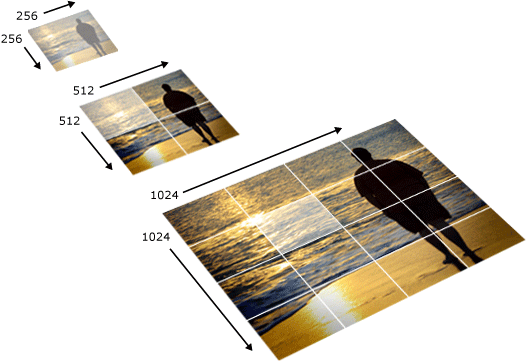
\includegraphics[scale=0.4]{img/dzi_pyramid.png}
		\caption{DZI pyramid model example (source:\cite{web:dzi})}
		\label{fig:fig2.2}
	\end{center}
\end{figure}

A DZI consists of two main parts\cite{web:dzi}: 
\begin{enumerate}[(1)]
	\item a describing XML file ([file name].dzi) with informations about:
	\begin{itemize}
		\item the format of single tiles (e.g. JPEG or PNG)
		\item overlap between tiles
		\item size of tiles
		\item height and width of baseline image
	\end{itemize}
	\item a directory ([file name]{\textunderscore}files) with image tiles of the specified format
\end{enumerate}

(1) and (2) are stored "next" to each other, so that there are 2 spearate files. (2) contains sub directories, one for each level of the image pyramid. The baseline image of a DZI is in the highest level. Each level is tessellated into as many tiles necessary to go over the whole image, with each tile having the size specified in the XML file. If the image size is no multiple of the specified tile size, the width of the $n^{th}$ column of tiles will be $(width \mod tile$ $size)$ pixels. Equally, the height of the $m^{th}$ row will be $(height \mod tile$ $size)$ pixels. Thus, the outermost right bottom tile $t_{n,m}$ will be of $(width \mod tile$ $size)$ x $(height \mod tile$ $size)$ pixels.


\subsubsection{International Image Interoperability Framework}
The International Image Interoperability Framework (IIIF)\nmc{IIIF}{International Image Interoperability Framework} is the result of a cooperation between The British Library, Stanford University, the Bodleian Libraries\footnote{Oxford University}, the Bibliothèque Nationale de France, Nasjonalbiblioteket\footnote{National Library of Norway}], Los Alamos National Laboratory Research Library and Cornell University\cite{Cramer11}. Version 1.0 was published in 2012.

IIIFs goal is to collaboratively produce an interoperable technology and community framework for image delivery\cite{web:iiif2}. To achieve this, IIIF tries to:
\begin{enumerate}[(1)]
	\item give scholars access to image-based resources around the world
	\item define a set of common APIs to support interoperability between image repositories
	\item develop and document shared technologies (such as image servers and web clients), that enable scholars to view, compare, manipulate and annotate images
\end{enumerate}

\begin{figure}[H]
	\begin{center}
		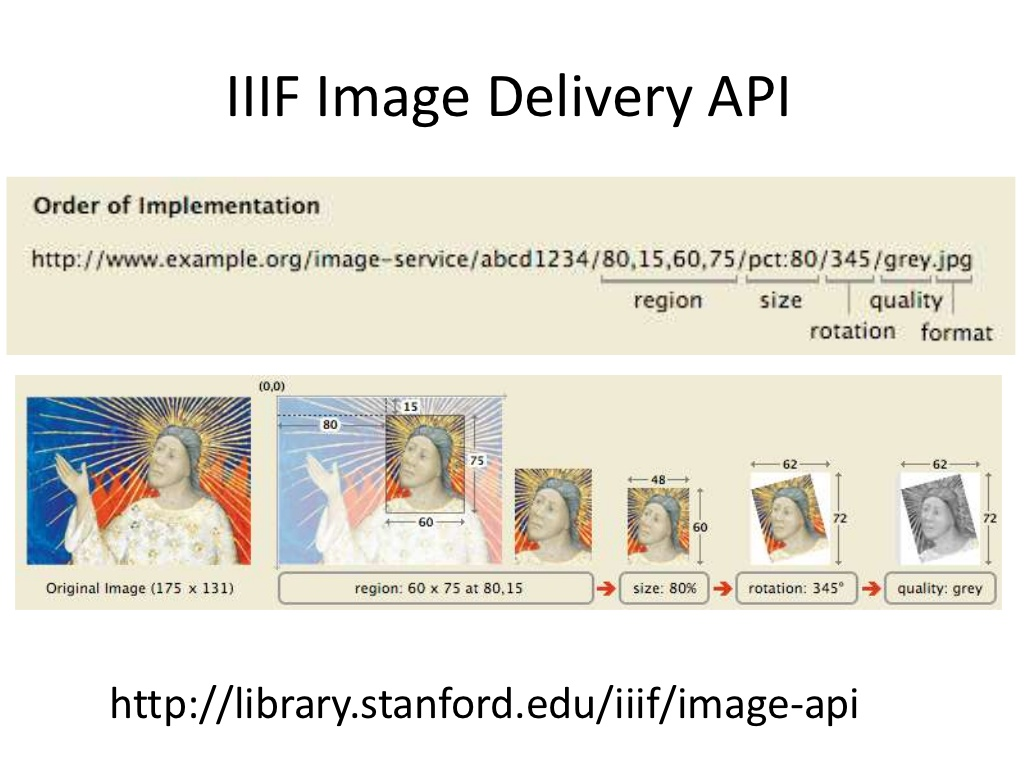
\includegraphics[scale=0.3]{img/iiif_url_example.jpg}
		\caption{Example of iiif request (source:\url{http://www.slideshare.net/Tom-Cramer/iiif-international-image-interoperability-framework-dlf2012?ref=https://www.diglib.org/forums/2012forum/transcending-silos-leveraging-linked-data-and-open-image-apis-for-collaborative-access-to-digital-facsimiles/})}
		\label{fig:fig2.3}
	\end{center}
\end{figure}

The relevant part for this thesis is (2), especially the image API\cite{web:iiif}. It specifies a web service that returns an image in response to a standard web request. The URL can specify the region, size, rotation, quality and format of the requested image (see fig. 2.3). Originally intended for resources in digital image repositories maintained by cultural heritage organizations, the API can be used to retrieve static images in response to a properly constructed URL\cite{web:openseadragon}. The URL scheme looks like this\cite{web:iiif}:
\begin{lstlisting}
{scheme}://{server}{/prefix}/{identifier}/{region}/{size}/{rotation}/{quality}.{format}
\end{lstlisting}

The \emph{region} and \emph{size} parameters are of special interest for this thesis\footnote{For detailed information on all parameters see the official API: \url{http://iiif.io/api/image/2.0}}. With them, it is possible to request only a certain region of an image in a specified size.

The region parameter defines the rectangular portion of the full image to be returned. It can be specified by pixel coordinates, percentage or by the value “full” (see tab. 2.2 and fig. 2.4).

\begin{table}[H]
	\begin{center}
		\begin{tabular}{| p{2cm} | p{9cm} |}
			\hline
			\textbf{Form} & \textbf{Description}\\ \hline
			full & The complete image is returned, without any cropping.\\ \hline
			x,y,w,h & The region of the full image to be returned is defined in terms of absolute pixel values. The value of x represents the number of pixels from the 0 position on the horizontal axis. The value of y represents the number of pixels from the 0 position on the vertical axis. Thus the x,y position 0,0 is the upper left-most pixel of the image. w represents the width of the region and h represents the height of the region in pixels.\\ \hline
			pct:x,y,w,h & The region to be returned is specified as a sequence of percentages of the full image’s dimensions, as reported in the Image Information document. Thus, x represents the number of pixels from the 0 position on the horizontal axis, calculated as a percentage of the reported width. w represents the width of the region, also calculated as a percentage of the reported width. The same applies to y and h respectively. These may be floating point numbers.\\ \hline
		\end{tabular}
		\caption{Valid values for \emph{region} parameter (source:\cite{web:iiif})}
	\end{center}
\end{table}

If the request specifies a regions whose size extends beyond the actual size of the image, the response should be a cropped image, instead of an image with added empty space. If the region is completely outside of the image, the response should be a 404 http status code\cite{web:iiif}.

\begin{figure}[H]
	\begin{center}
		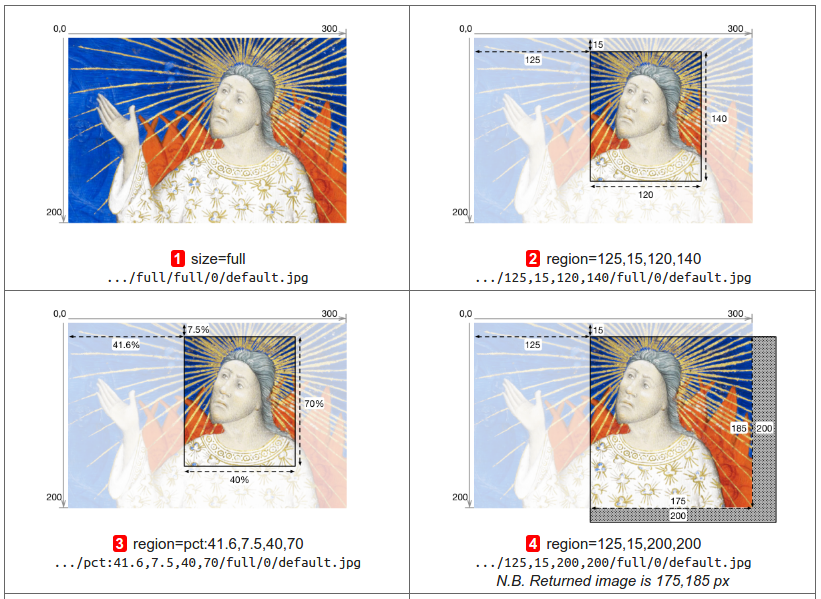
\includegraphics[scale=0.4]{img/region_param.png}
		\caption{Results of IIIF request with different values for region parameter (source:\cite{web:iiif})}
		\label{fig:fig2.4}
	\end{center}
\end{figure}

If a region was extracted, it is scaled to the dimensions specified by the size parameter (see tab. 2.3 and fig. 2.5).

\begin{figure}[H]
	\begin{center}
		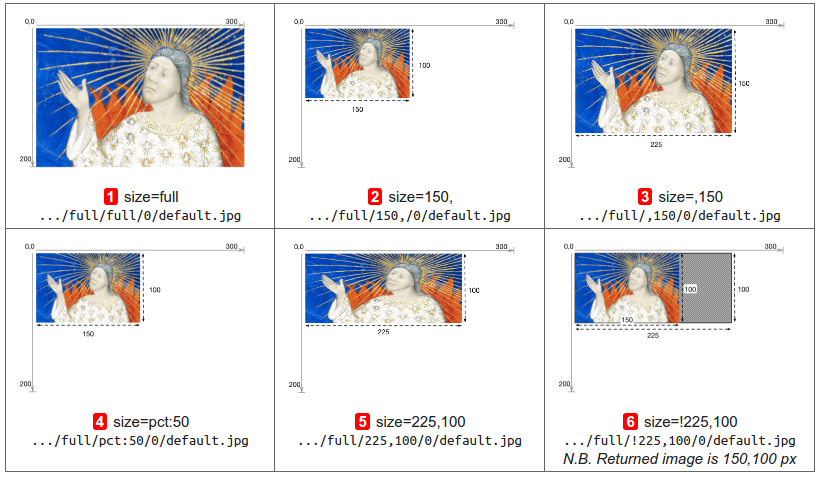
\includegraphics[scale=0.35]{img/size_parameter.png}
		\caption{Results of IIIF request with different values for size parameter (source:\cite{web:iiif})}
		\label{fig:fig2.5}
	\end{center}
\end{figure}

If the resulting height or width equals 0, then the server should return a 400 http status code. Depending on the image server, scaling above the full size of the extracted region may be supported\cite{web:iiif}.

\begin{table}[H]
	\begin{center}
		\begin{tabular}{| p{2cm} | p{9cm} |}
			\hline
			\textbf{Form} & \textbf{Description}\\ \hline
			full & The extracted region is not scaled, and is returned at its full size.\\ \hline
			w, & The extracted region should be scaled so that its width is exactly equal to w, and the height will be a calculated value that maintains the aspect ratio of the extracted region.\\ \hline
			,h & The extracted region should be scaled so that its height is exactly equal to h, and the width will be a calculated value that maintains the aspect ratio of the extracted region.\\ \hline
			pct:n & The width and height of the returned image is scaled to n\% of the width and height of the extracted region. The aspect ratio of the returned image is the same as that of the extracted region.\\ \hline
			w,h & The width and height of the returned image are exactly w and h. The aspect ratio of the returned image may be different than the extracted region, resulting in a distorted image.\\ \hline
			!w,h & The image content is scaled for the best fit such that the resulting width and height are less than or equal to the requested width and height. The exact scaling may be determined by the service provider, based on characteristics including image quality and system performance. The dimensions of the returned image content are calculated to maintain the aspect ratio of the extracted region.\\ \hline
		\end{tabular}
		\caption{Valid values for \emph{size} parameter (source:\cite{web:iiif})}
	\end{center}
\end{table}

To use the IIIF API, a compliant web server must be deployed. There are 2 alternatives to set up a new one\cite{web:openseadragon},\cite{web:iiif2}:
\begin{itemize}
	\item \textbf{Loris}, an open source image server based on python that supports the IIIF API versions 2.0, 1.1 and 1.0. Supported image formats are JPEG, JPEG2000 and TIFF.
	\item \textbf{IIPImage Server}, an open source Fast CGI module written in C++, that is designed to be embedded within a hosting web server such as Apache, Lighttpd, MyServer or Nginx. Supported image formats are JPEG2000 and TIFF.
\end{itemize}

\subsubsection{OpenStreetMap/Tiled Map Service}
OpenStreetMap (OSM)\nmc{OSM}{OpenStreetMap} is a popular tile source used in many online geographic mapping specifications\cite{web:openseadragon}. It's a community driven alternative to services such as Google Maps. Information is added by users via aerial images, GPS devices and field maps. All OSM data is classified as \emph{open data}, meaning that it can be used anywhere, as long as the OSM Foundation is credited\cite{web:osm}.

Tiled Map Service (TMS)\nmc{TMS}{Tiled Map Service} is a tile scheme developed by the Open Source Geospatial Foundation (OSGF)\nmc{OSGF}{Open Source Geospatial Foundation}\cite{web:openseadragon} and specified in \cite{web:tms}. The OSGF is a nonprofit organization whose goal it is to support the needs of the open source geospatial community. TMS provides access to cartographic maps of geo-referenced data. Access to these resources is provided via a "REST" interface, starting with a root resource describing available layers, then map resources with a set of scales, then scales holding sets of tiles\cite{web:tms}.

Both, OSM and TMS, offer zooming images, which in general, have the functionality necessary, to be of use for this thesis. Unfortunately, the are also highly specialized on the needs of the mapping community, which makes them unattractive choices for the research objective of this thesis respectively.


\subsubsection{JPEG 2000}
\cite{web:jpeg2000} describes the image compression standard JPEG 2000 as follows:
\begin{quotation}
	"JPEG 2000 is an image coding system that uses state-of-the-art compression techniques based on wavelet technology. Its architecture lends itself to a wide range of uses from portable digital cameras through to advanced pre-press, medical imaging and other key sectors."
\end{quotation}

It incorporates a mathematically lossless compression mode, in which the storage requirement of images can be reduced by an average of 2:1. On top of that, there is a visually lossless compression rate\footnote{At \emph{At visually lossless compression rates, even a trained a can't see the difference between original and compressed version\cite{intoPix08}.}} of between 10:1 to 20:1\cite{intoPix08}. JPEG 2000 code streams offer mechanisms to support random access at varying degrees of granularity. It is possible to store different parts of the same picture using different quality\cite{Taubmann01}. 

In the compression process, JPEG 2000 partitions an image into rectangular and non-overlapping tiles of equal size (except for tiles at the image borders). The tile size is arbitrary and
can be as large as the original image itself (resulting in only one tile) or as small as a single pixel. Furthermore, the image gets decomposed into a multiple resolution representation\cite{Rabbani02}. 

This creates a tiled image pyramid, similar to the one described in \cite{DICOM10}.

The encoding-decoding process of JPEG 2000 is beyond the scope of this thesis. Therefore, it is recommended to consult either \cite{intoPix08} for a quick overview or \cite{Rabbani02} for an in depth guide.


\subsubsection{TIFF/BigTIFF}
The Tagged Image File Format (TIFF)\nmc{TIFF}{Tagged Image File Format} consists of a number of corresponding key-value pairs (e.g. \emph{ImageWidth} and \emph{ImageLength}, who describe the width and length of contained the image), called \emph{tags}. One of the core features of this format is that it allows for the image data to be stored in tiles\cite{Eddins07}.

Each tiles offset is saved in an image header, so that efficient random access to any tile is granted. The original specification demands a use of 32 bit file offset values, limiting the maximum offset to $2^{32}$. This constraint limits the file size to be below 4 GB\cite{Eddins07}.

This constraint lead to the development of BigTIFF. The offset values were raised to a 64 bit base, limiting the maximum offset to $2^{64}$. This results in an image size of up to 18,000 peta bytes\cite{web:digitalpreservation}.

TIFF and BigTIFF are capable of saving images in multiple resolutions. Together with the feature of saving tiles, the image pyramid model described in \cite{DICOM10} can be used in BigTIFF/TIFF images\cite{web:digitalpreservation2}.


\subsection{Choice of Format}



\section{Short Introduction to Neural Networks}
The objective of this thesis ultimately is to create training samples for NN\footnote{compare chap. 1.2}. Before going into other details, it is necessary to clarify what NN are, how they work, why they need training samples and what they use them for\footnote{It should be mentioned that the scope of NN is huge and worth a whole thesis by themselves. This is nothing more than a short introduction and further consultation of literature (e.g. \cite{Stergiou96},\cite{Bourg04},\cite{Egmont-Petersen02},\cite{Kriesel07},\cite{Shiffman12}) is highly recommended.}.

Artificial Neural Networks (NN)\nmc{NN}{Neural Networks} are a group of models inspired by Biological Neural Networks (BNN) \nmc{BNN}{Biological Neural Networks}. BNNs can be described as an interconnected web of neurons (see fig 2.x), whose purpose it is to transmit information in the form of electrical signals. A neuron receives input via dendrites and send output via axons\cite{Shiffman12}. An average human adult brain contains about $10^{11}$ neurons. Each of those receives input from about $10^4$ other neurons. If their combined input is strong enough, the receiving neuron will send an output signal to other neurons\cite{Bourg04}.

\begin{figure}[H]
	\begin{center}
		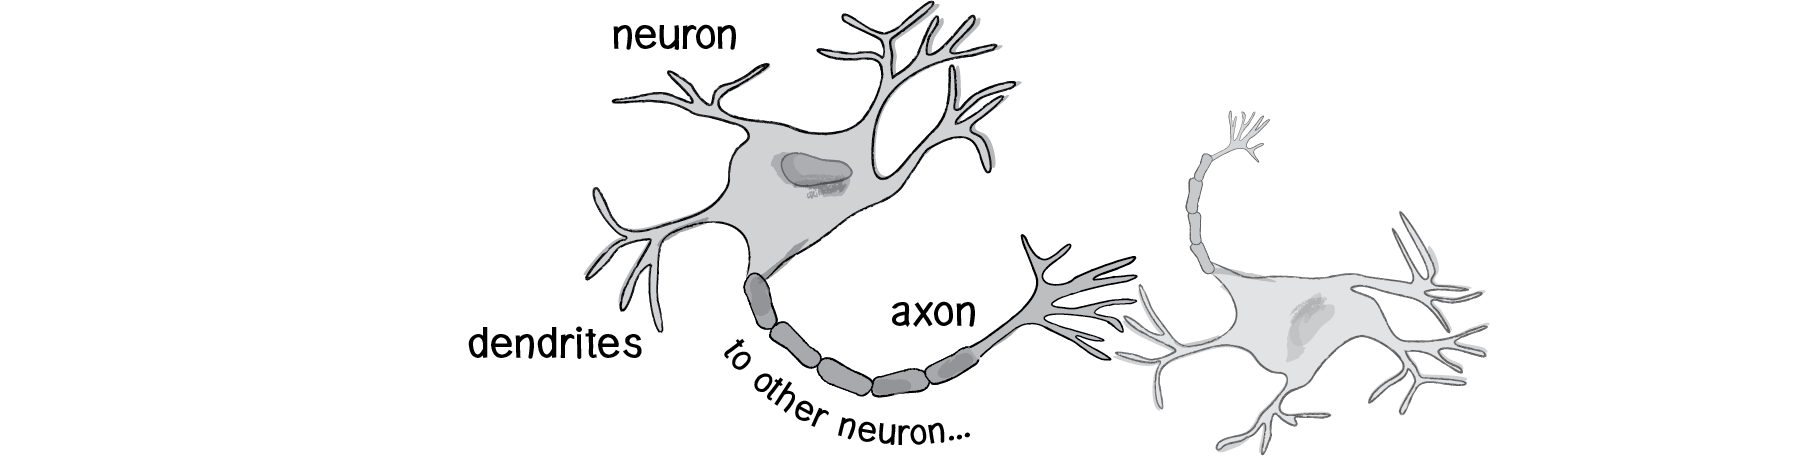
\includegraphics[scale=0.7]{img/bnn.png}
		\caption{Neuron in a BNN (source:\cite{Shiffman12})}
		\label{fig:fig2.2}
	\end{center}
\end{figure}

NN are much simpler in comparison\footnote{Usually, they don't have much more than a few dozen neurons\cite{Bourg04}.}, but generally work in the same fashion.

One of the biggest strengths of a NN, much like a BNN, is the ability to adapt by learning\footnote{As humans, NN learn by training\cite{Shiffman12}.}. This adaption is based on \emph{weights} that are assigned to the connections between single neurons. Fig 2.x shows an exemplary NN with neurons and the connections between them.

\begin{figure}[H]
	\begin{center}
		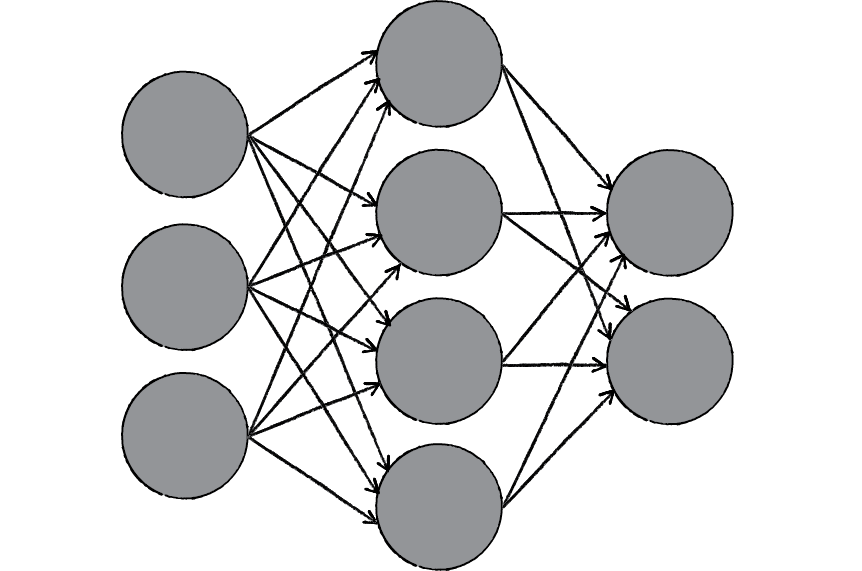
\includegraphics[scale=1.0]{img/NN.png}
		\caption{Exemplary NN (source:\cite{Shiffman12})}
		\label{fig:fig2.3}
	\end{center}
\end{figure}

Each line in fig, 2.x represents a connection between 2 neurons. Those connections are a one-directional flow of information, each assigned with a specific weight. This weight is a simple number that is multiplied with the incoming/outgoing signal and therefore weakens or enhances it. They are the defining factor of the behavior of a NN. Determining those values is the purpose of training a NN\cite{Bourg04}.

According to \cite{Shiffman12}, some of the standard use cases for NN are:

\begin{itemize}
	\item Pattern Recognition
	\item Time Series Prediction
	\item Signal Processing Perceptron
	\item Control
	\item Soft Sensors
	\item Anomaly Detection
\end{itemize}


\subsection{Methods of Learning}
There are 3 general strategies when it comes to the training of a NN\cite{Bourg04}. Those are:

\begin{enumerate}
	\item Supervised Learning
	\item Unsupervised Learning
	\item Reinforcement Learning (a variant of Unsupervised Learning\cite{Rojas96})
\end{enumerate}

\emph{Supervised Learning} is a strategy that involves a training set to which the correct output is known, as well as an observing teacher. The NN is provided with the training data and computes its output. This output is compared to the expected output and the difference is measured. According to the error made, the weights of the NN are corrected. The magnitude of the correction is determined by the used learning algorithm\cite{Rojas96}.

\emph{Unsupervised Learning} is a strategy that is required when the correct output is unknown and no teacher is available. Because of this, he NN must organize itself\cite{Shiffman12}. \cite{Rojas96} makes a distinction between 2 different classes of unsupervised learning:

\begin{itemize}
	\item reinforced learning
	\item competitive learning
\end{itemize}

Reinforced learning adjusts the weights in such a way, that desired output is reproduced. For example, a robot in a maze. If the robot can drive straight without any hindrances, it can associate this sensory input with driving straight (desired outcome). As soon as it approaches a turn, the robot will hit a wall (non-desired outcome). To prevent it from hitting the wall it must turn, therefore the weights of turning must be adjusted to the sensory input of being at a turn. Another example is \emph{Hebbian learning}\footnote{see \cite{Rojas96} for further information}\cite{Rojas96}.

In competitive learning, the single neurons compete against each other for the right to give a certain output for an associated input. Only one element in the NN is allowed to answer, so that other, competing neurons are inhibited\cite{Rojas96}.


\subsection{The Perceptron}
The perceptron was invented by Rosenblatt at the Cornell Aeronautical Laboratory in 1957\cite{Rosenblatt58}. It is the computational model of a single neuron and as such, the simplest NN possible\cite{Shiffman12}. A perceptron consists of one or more inputs, a processor and a single output (see fig. 2.x)\cite{Rosenblatt58}.

\begin{figure}[H]
	\begin{center}
		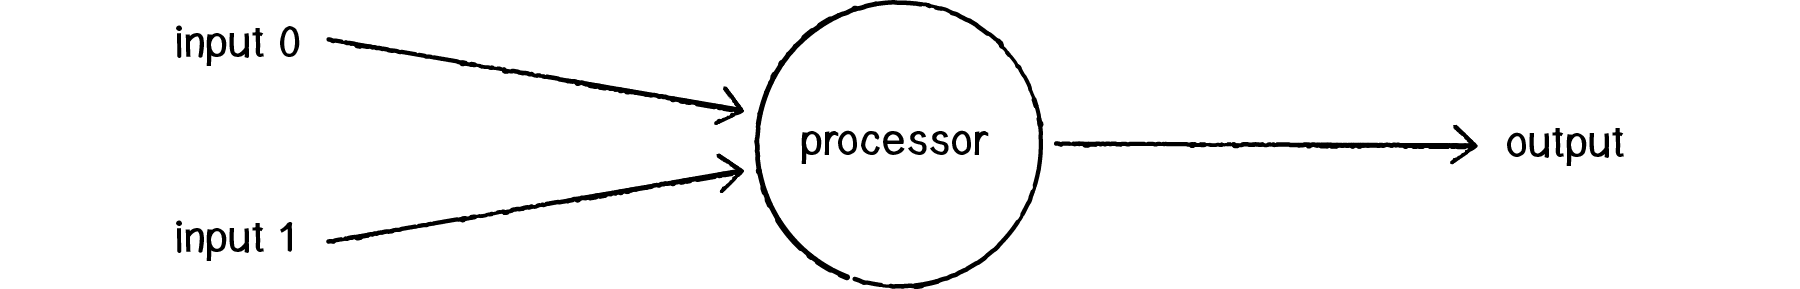
\includegraphics[scale=0.7]{img/perceptron.png}
		\caption{Perceptron by Rosenblatt (source:\cite{Shiffman12})}
		\label{fig:fig2.5}
	\end{center}
\end{figure}

This can be directly compared to the neuron in fig. 2.x, where:
\begin{itemize}
	\item input = dendrites
	\item processor = cell
	\item output = axon
\end{itemize}

A perceptron is only capable of solving \emph{linearly separable} problems, such as logical \emph{AND} and \emph{OR} problems. To solve non-linearly separable problems, more then one perceptron is required\cite{Rosenblatt58}. Simply put, a problem is linearly separable, if it can be solved with a straight line (see fig. 2.x), otherwise it is considered a non-linearly separable problem (see fig. 2.x).

\begin{figure}[H]
	\begin{center}
		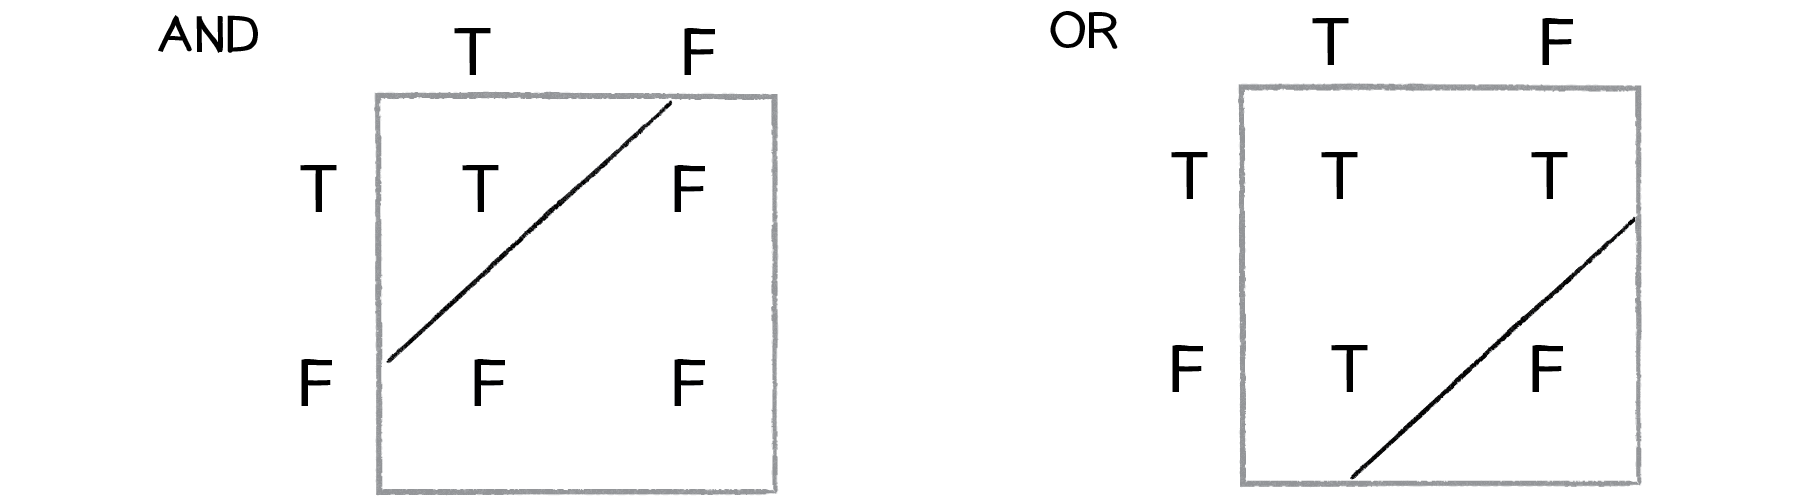
\includegraphics[scale=0.6]{img/lsp.png}
		\caption{Examples for linearly separable problems (source:\cite{Shiffman12})}
		\label{fig:fig2.7}
	\end{center}
\end{figure}

\begin{figure}[H]
	\begin{center}
		
\includegraphics[scale=0.75]{img/nlsp.png}
		\caption{Examples for non-linearly separable problems (source:\cite{Shiffman12})}
		\label{fig:fig2.8}
	\end{center}
\end{figure}


\subsection{Multi-layered Neural Networks}
To solve more complex problems, multiple perceptrons can be connected to from a more powerful NN. A single perceptron might not be able to solve \emph{XOR}, but one perceptron can solve \emph{OR}, while the other can solve \emph{$\neg$AND}. Those two perceptrons combined can solve \emph{XOR}\cite{Shiffman12}.

If multiple perceptrons get combined, they create layers. Those layers can be separated into 3 distinct types\cite{Stergiou96}:
\begin{itemize}
	\item input layer
	\item hidden layer
	\item output layer
\end{itemize}

A typical NN will have an input layer, which is connected to a number of hidden layers, which either connect to more hidden layers or, eventually, an output layer (see fig. 2.x for a NN with one hidden layer).

\begin{figure}[H]
	\begin{center}
		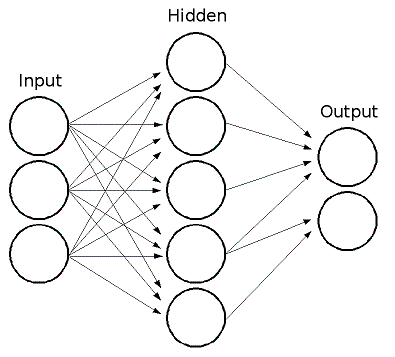
\includegraphics[scale=0.8]{img/mlp.png}
		\caption{NN with multiple layers (source: \url{http://docs.opencv.org/2.4/_images/mlp.png)}}
		\label{fig:fig2.2}
	\end{center}
\end{figure}

As the name suggests, the input layer gets provided with the raw information input. Depending on the internal weights and connections inside the hidden layer, a representation of the input information gets formed. At last, the output layer generates output, again based on the connections and weights of the hidden and output layer\cite{Stergiou96}.

Training this kind of NN is much more complicated than training a simple perceptron, since weights are scattered all over the NN and its layers. A solution to this problem is called \emph{backpropagation}\cite{Shiffman12}.


\subsubsection{Backpropagation}
Training is an optimization process. To optimize something, a metric to measure has to be established. In the case of backpropagation, this metric is the accumulated output error of the NN to a given input\footnote{To do so, it is necessary to know the right answer. Therefore, backpropagation is part of the supervised learning process.}. There are several ways to calculate this error, with the \emph{mean square error}\footnote{Mean square error is the average of the square of the differences of two variables, in this case the expected and the actual output.} being the most common one\cite{Bourg04}.

Finding the optimal weights is an iterative process of the following steps:
\begin{enumerate}
	\item start with training set of data with known output
	\item initialize weights in NN
	\item for each set of input, feed the NN and compute the output
	\item compare calculated with known output
	\item adjust weights to reduce error
\end{enumerate}

There are 2 possibilities in how to proceed. The first one is to compare results and adjust weights after each input/output-cycle. The second one is to calculate the accumulated error over a whole iteration of the input/output-cycle. Each of those iterations is known as an \emph{epoch}\cite{Bourg04}.


\section{Microservices}
The following section elaborates on the concept of \emph{Microservices} (MS)\nmc{MS}{Microservice}, defining what they are, listing their pros and cons, as well as explaining why this approach was chosen over a monolithic approach. A monolithic software solution is described by \cite{Lewis14} as follows:
\begin{quotation}
	"[...] a monolithic application [is] built as a single unit. Enterprise Applications are often built in three main parts: a client-side user interface (consisting of HTML pages and javascript running in a browser on the user's machine) a database (consisting of many tables inserted into a common, and usually relational, database management system), and a server-side application. The server-side application will handle HTTP requests, execute domain logic, retrieve and update data from the database, and select and populate HTML views to be sent to the browser. This server-side application is a monolith - a single logical executable. Any changes to the system involve building and deploying a new version of the server-side application."
\end{quotation}


\subsection{Definition}
MS are an interpretation of the Service Oriented Architecture. The concept is to separate one monolithic software construct into several smaller, modular pieces of software\cite{Wolff16}. As such, MS are a modularization concept. However, they differ from other such concepts, since MS are independent from each other. This is a trait, other modularization concepts usually lack\cite{Wolff16}. As a result, changes in one MS don't bring up the necessity of deploying the whole product cycle again, but just the one service. This can be achieved by turning each MS into an independent process with its own runtime\cite{Lewis14}.

This modularization creates an information barrier between different MS. Therefore, if MS need to share data or communicate with each other, light weight communication mechanisms must be established, such as a RESTful API\cite{Riggins15}.

Even though MS are more a concept than a specific architectural style, certain traits are usually shared between them\cite{Riggins15}. According to \cite{Riggins15} and \cite{Lewis14}, those are:

\begin{enumerate}[(a)]
	\item \textbf{Componentization as a Service:} bringing chosen components (e.g. external libraries) together to make a customized service
	\item \textbf{Organized Around Business Capabilities:} cross-functional teams, including the full range of skills required to achieve the MS goal
	\item \textbf{Products instead of Projects:} teams own a product over its full lifetime, not just for the remainder of a project
	\item \textbf{Smart Endpoints and Dumb Pipes:} each microservice is as decoupled as possible with its own domain logic
	\item \textbf{Decentralized Governance:} enabling developer choice to build on preferred languages for each component.
	\item \textbf{Decentralized Data Management:} having each microservice label and handle data differently
	\item \textbf{Infrastructure Automation:} including automated deployment up the pipeline
	\item \textbf{Design for Failure:} a consequence of using services as components, is that applications need to be designed so that they can tolerate the failure of single or multiple services
\end{enumerate}

Furthermore, \cite{Bugwadia15} defined 5 architectural constraints, which should help to develop a MS:

\begin{enumerate}[(1.)]
	\item \textbf{Elastic}\\
	The elasticity constraint describes the ability of a MS to scale up or down, without affecting the rest of the system. This can be realized in different ways. \cite{Bugwadia15} suggests to architect the system in such a fashion, that multiple stateless instances of each microservice can run, together with a mechanism for Service naming, registration, and discovery along with routing and load-balancing of requests.
	\item \textbf{Resilient}\\
	This constraint is referring to the before mentioned trait (h) - \emph{Design for Failure}. The failure of or an error in the execution of a MS must not impact other services in the system.
	\item \textbf{Composable}\\
	To avoid confusion, different MS in a system should have the same way of identifying, representing, and manipulating resources, describing the API schema and supported API operations.
	\item \textbf{Minimal}\\
	A MS should only perform one single business function, in which only semantically closely related components are needed.
	\item \textbf{Complete}\\
	A MS must offer a complete functionality, with minimal dependencies to other services. Without this constraint, services would be interconnected again, making it impossible to upgrade or scale individual services.
\end{enumerate}


\subsection{Advantages and Disadvantages}
% pros
One big advantage of this modularization is that each service can be written in a different programming language, using different frameworks and tools. Furthermore, each microservice can bring along its own support services and data storages. It is imperative for the concept of modularization, that each microservice has its own storage of which it is in charge of\cite{Wolff16}.

The small and focused nature of MS makes scaling, updates, general changes and the deploying process easier. Furthermore, smaller teams can work on smaller code bases, making the distribution of know how easier\cite{Riggins15}.

Another advantage is how well MS plays into the hands of agile, scrum and continuous software development processes, due to their previously discussed inherent traits.

% cons
The modularization of MS doesn't only yield advantages. Since each MS has its own, closed off data management\footnote{See 2.3.1(f) (\emph{Decentralized Data Management})}, interprocess communication becomes a necessity. This can lead to communicational overhead which has a negative impact on the overall performance of the system\cite{Wolff16}.

2.3.1(e) (\emph{Decentralized Governance}) can lead to compatibility issues, if different developer teams chose to use different technologies. Thus, more communication and social compatibility between teams is required. This can lead to an unstable system which makes the deployment of extensive workarounds necessary\cite{Riggins15}.

It often makes sense to share code inside a system to not replicate functionality which is already there and therefore increase the maintenance burden. The independent nature of MS can make that very difficult, since shared libraries must be build carefully and with the fact in mind, that different MS may use different technologies, possibly creating dependency conflicts.


\subsection{Conclusion}	
After consideration of the advantages and disadvantages of MS, the author decided in favor of using them. This is mainly due to the fact of working alone on the project, negating some of their inherent disadvantages:
\begin{itemize}
	\item Interprocess communication doesn't arise between the single stages of the process chain, since they have a set order\footnote{E.g. it wouldn't make sense trying extract a training sample without converting or annotating a WSI first.}
	\item Different technologies may be chosen for the single steps of the process chain, however, working alone on the project makes technological incompatibilities instantly visible
	\item The services shouldn't share functionality, therefore there should be no need for shared libraries
\end{itemize}
This makes the advantages outweight the disadvantages clearly:
\begin{itemize}
	\item different languages and technologies can be used for every single step of the process chain, making the choice of the most fitting tool possible
	\item WSIs take a heavy toll on memory and disk space due to their size; the use of MS allows each step of the chain to handle those issues in the most suitable way for each given step
	\item separating the steps of the process chain into multiple MS makes for a smaller and easier maintainable code base
	\item other bachelor/master students may continue to use or work on this project in the future, making the benefit of a small, easily maintainable code base twice as important
	\item the implementation of the project will happen in an iterative, continuous manner, which is easily doable with the use of MS
\end{itemize}


\section{Process Chain}
This section and its following subsections are dedicated to establish the process chain necessary to accomplish the research objectives stated in 1.2(a) - 1.2(c). The usual procedure would look as follows:

\begin{enumerate}[(1.)]
	\item convert chosen WSI $img^{wsi}_i$ to DZI format $img^{dzi}_i$
	\item open $img^{dzi}_i$ in a viewer $V$
	\item annotate $img^{dzi}_i$ in $V$
	\item persist annotations $A_i$ on $img^{dzi}_i$ in a file $f_{(A_i)}$
	\item create training sample $ts_i$ by extracting the information of $A_i$ in correspondence to $img^{dzi}_i$
\end{enumerate}

While it only makes sense to run (1.) once per $img^{wsi}_i$ to create $img^{dzi}_i$, steps (2.) - (4.) can be repeated multiple times, so that there is no need to finish the annotation of an image in one session. That makes it necessary to not only save but also load annotations. Therefore, the loading of already made annotations can be added as step (2.5). This also enables the user of editing and deleting already made annotations. Because of this, step (5.) also needs to be repeatable.

The single steps of the process chain will be sorted into semantic groups. Each group will be realized by its own MS, as stated in 2.3. The semantic groups are: conversion (1.), extraction (5.) and viewing and annotation (2. - 4.).

A MS will be introduced for each group in the following subsections(2.4.1 - 2.4.3). Those are:

\begin{itemize}
	\item \textbf{Conversion Service}\\
	This service will be responsible of the conversion from $img^{wsi}_i$ to $img^{dzi}_i$ (1.).
	\item \textbf{Annotation Service}\\
	This service will offer a GUI to view a $img^{dzi}_i$, as well as make and manage annotations (2. - 4.)
	\item \textbf{Tessellation Service}\\
	This service will be responsible for extracting a $ts_i$ from a given $A_i$ and $img^{dzi}_i$ (5.).
\end{itemize}


\subsection{Conversion Service}

The devices which create WSIs, so called \emph{whole slide scanners}, create images in various formats, depending on the producer and a lack of a defined standard\cite{Cornish13}. The Conversion Service (CS)\nmc{CS}{Conversion Service} has the goal of converting those formats to DZI\footnote{see chap. 1.2(i) and 1.2(ii) for the reasons}].

\begin{figure}[H]
	\begin{center}
		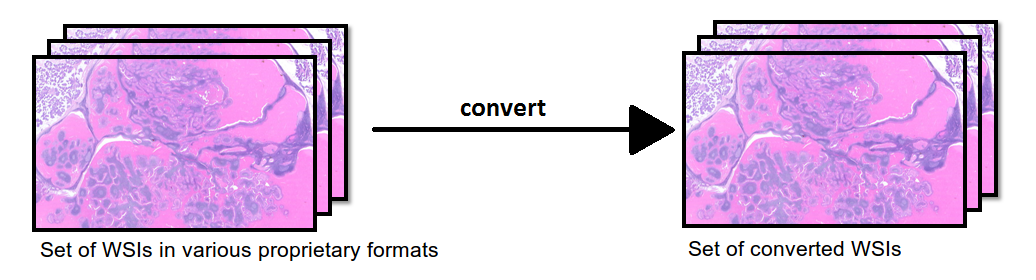
\includegraphics[scale=0.35]{img/processChainA.png}
		\caption{Visualization of the Conversion Service}
		\label{fig:fig2.1}
	\end{center}
\end{figure}

Upon invocation, the CS will take every single WSI inside a given directory and convert it to DZI. The output of each conversion will be saved in another specified folder. Valid image formats for conversion are:

\begin{itemize}
	\item .bif
	\item .mrxs
	\item .ndpi
	\item .scn
	\item .svs
	\item .svslide
	\item .tif
	\item .tiff
	\item .vms
	\item .vmu
\end{itemize}


\subsection{Annotation Service}
As mentioned in 2.4, the Annotation Service (AS)\nmc{AS}{Annotation Service} will provide a graphical user interface (GUI)\nmc{GUI}{Graphical User Interface} to view a DZI, make annotations and manage those annotations. This also includes persisting made annotations in a file (see fig. 2.2).

\begin{figure}[H]
	\begin{center}
		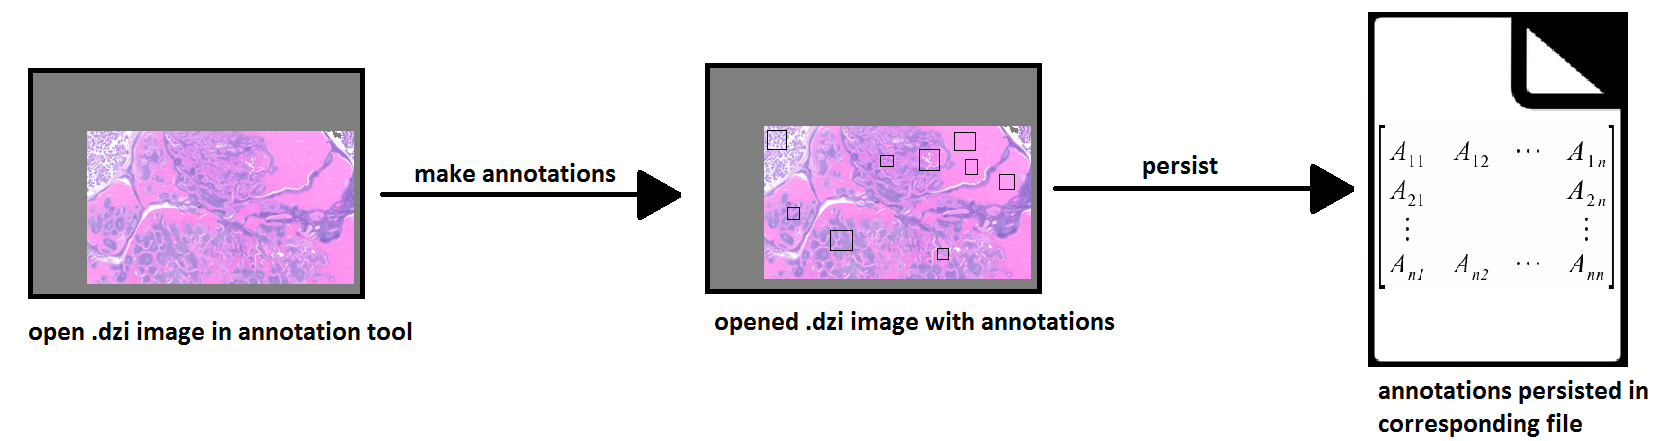
\includegraphics[scale=0.25]{img/processChainB.png}
		\caption{Visualization of the Annotation Service}
		\label{fig:fig2.4}
	\end{center}
\end{figure}

The supplied GUI will offer different tools to help the user annotate the DZI, e.g. a ruler to measure the distance between 2 points. The annotations themselves will be made via drawing a contour around an object of interest and putting a specified label to that region. To ensure uniformity of annotations, labels will not be added in free text. Instead they will be selected from a predefined dictionary.


\subsection{Tessellation Service}

The task of the Tessellation Service (TS)\nmc{TS}{Tessellation Service} is to extract annotations and their corresponding image data in such a fashion that they will become usable as training samples for NN.

\begin{figure}[H]
	\begin{center}
		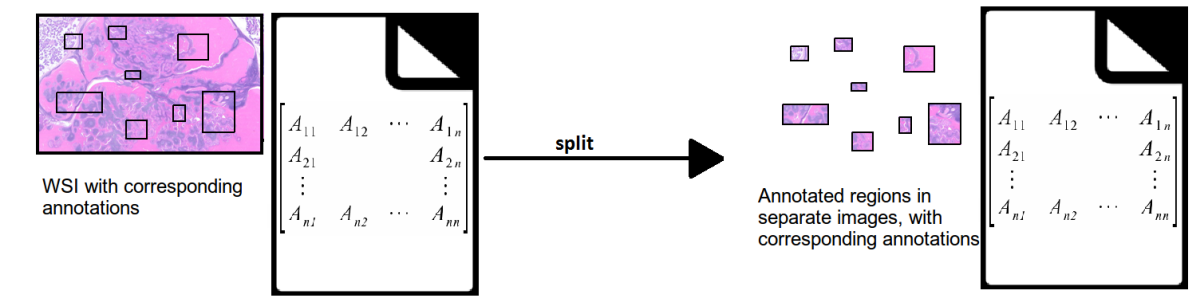
\includegraphics[scale=0.3]{img/processChainC.png}
		\caption{Visualization of the Tessellation Service}
		\label{fig:fig2.6}
	\end{center}
\end{figure}

Let there be a DZI $D$ and a corresponding set of annotations $A$. The TS will achieve the extraction by iterating over every $a_i \in A$, creating a sub-image $d_i$ which is the smallest bounding box around the region described by $a_i$ (see fig. 2.3). To be used as training sample, the TS must keep up the correspondence between $d_i$ and $a_i$.